% Chapter 1

\chapter{Hand segmentation in ego-centric videos}

\lhead{Chapter 3. \emph{Hand segmentation}} % This is for the header on each page - perhaps a shortened title

%----------------------------------------------------------------------------------------
We now focus on the task of pixel-wise hand detection
from video recorded with a wearable head-mounted
camera. In contrast to a third-person point-of-view camera,
such as a mounted surveillance camera or a TV camera,
a first-person point-of-view wearable camera has exclusive
access to first-person activities and is an ideal viewing perspective
for analyzing fine motor skills such as hand-object
manipulation or hand-eye coordination. As we said before, the use of
ego-centric video has re-emerged as a popular topic in computer
vision and has shown promising results in such areas
as understanding hand-eye coordination and recognizing
activities of daily living. In order to achieve more
detailed models of human interaction and object manipulation, and, in our case, to perform hand gesture recognition,
it is important to detect hand regions with pixel-level
accuracy. Hand detection is, in fact, an important element of such
tasks as gesture recognition, hand tracking, grasp recognition,
action recognition and understanding hand-object interactions.

The egocentric
paradigm presents a new set of constraints and characteristics
that introduce new challenges as well as unique
properties that can be exploited for the task of first-person
hand detection. Unlike static third-person point-of-view
cameras typically used for gesture recognition or sign language
analysis, the video acquired by a first-person camera
undergoes large ego-motion because it is worn by the
user. The mobile nature of the camera also results in images
recorded over extreme transitions in lighting, such as
walking from indoors to outdoors. As a result, the large image displacement caused by body motion makes it very difficult
to apply traditional image stabilization or background
subtraction techniques. Similarly, large changes in illumination
conditions induce large fluctuations in the appearance
of hands. Fortunately, ego-centric videos also have the
property of being user-specific, where images of hands and
the physical world are always acquired with the same camera
for the same user. This implies that the intrinsic colour
of the hands does not change drastically over time.

The purpose of this chapter is to identify and address the
challenges of hand detection for first-person vision. To this
end, we present existing and recent hand detection approaches, and we propose a novel algorithm capable of facing
various illumination conditions and different backgrounds. Furthermore, we analyze our proposal on existing datasets to highlight the pros and cons of various widely-used local appearance features. We
evaluate the value of modeling global illumination to generate
an ensemble of hand region detectors conditioned on the
illumination conditions of the scene. Based on our finding,
we propose a model using sparse feature selection and an
illumination-dependent modeling strategy, and show that it
out-performs several baseline approaches.

\section{Previous approaches in Hand Segmentation}
The problem of hand detection  in ego-vision scenario, has been addressed only recently by the research community. Khan \etal's paper \cite{khan10}, for example, addresses skin detection as a general task for face detection and hand gesture analysis. They used the IHLS colour space for raw pixel based skin detection and evaluated different classifiers: Random Forest, Bayesian Networks, Multilayers Perceptrons, AdaBoost, Naive Bayes, RBF Networks. They demonstrated on a database of 8991 images that Random Forest classification obtains the highest F-score among all the other techniques. Also, they show the effect of increasing the number of trees: the maximum F-score is achieved with 10 trees, while an higher number of tree doesn't increase the F-score.

Jones \etal \cite{jones99} describe the construction of colour models for skin and non-skin classes from a dataset of nearly 1 billion labelled pixels. These classes exhibit a surprising degree of separability which we exploit by building a skin pixel detector achieving a detection rate of 80\% with 8.5\% false positives. They also compare the performance of histogram and mixture models in skin detection and find histogram models to be superior in accuracy and computational cost. Using aggregate features computed from the
skin pixel detector they build an effective detector for naked people. Their results suggest that colour can be the most powerful cue for detecting people in unconstrained imagery.

On a different note, Hayman \etal \cite{hayman03} propose a video stabilization approach for hand segmentation. They present a probabilistic
framework for when the camera pans and tilts. A unified approach is developed for handling various sources of error, including motion blur, sub-pixel camera motion, mixed pixels at object boundaries, and also uncertainty in background stabilisation caused by noise, unmodelled radial distortion and small translations of the camera. The second contribution regards a Bayesian approach to
specifically incorporate uncertainty concerning whether the background has yet been uncovered by moving foreground
objects. They don't assume that a background model is available in advance, instead they generate the background model online, very possibly in the presence of moving objects.

Fathi \etal \cite{fathi11} try to solve the hand segmentation problem in the ego-centric perspective, with a foreground segmentation approach. Their method is based on a few
assumptions: (1) that the background
is static in the world coordinate frame, (2) they define foreground
as every entity which is moving with respect to the
static background, (3) they assume background objects are
usually farther away from the camera than foreground objects
and (4) they assume they can build a panorama of the background scene by stitching the background images together
using an affine transformation. The fourth assumption
is basically assuming that the background is roughly
on a plane or far enough from the camera. An object will
be moving with respect to the background when it is being
manipulated by hands. When the subject finishes a sub-task
and stops manipulating the object, the object will become a
part of background again.

Their segmentation method is as follows. They first make an
initial estimate of background regions in each image by fitting
a fundamental matrix to dense optical flow vectors. They
make temporally local panoramas of background given their
initial background region estimates. Then they register each
image into its local background panorama. The regions in
the image which do not match the background scene are
likely to be parts of foreground. Then they connect the regions in
sequence of images spatially and temporally and use graphcut
to split them into foreground and background segments.
They split the video into short intervals and make local
background models for each. The reason is that the background
might change over time, for example the subject
might finish manipulating an object and leave it on the table,
letting it become a part of background. They initially approximately
separate foreground and background channels
for each image by fitting a fundamental matrix to its optical
flow vectors. They compute the flow vectors to its few adjacent
frames. For each interval we choose a reference frame
whose initial background aligns the best to other frames.

They build two kinds of temporally local models for background
(panoramas): (1) a model based on colour and texture
histogram of regions and (2) a model of region boundaries.
To build these models, they fit an affine transformation
to the initial background SIFT feature correspondences of
each frame in the interval, and the reference frame. They
stitch these images using affine transformation. After fixing
the images to the reference frame coordinate, they build
the colour-texture and boundary background models. This is
by computing a histogram of values extracted from interval
images corresponding to each location in the background
panorama.

On the other hand, Li and Kitani in \cite{li13} provide an historical overview about approaches for detecting hands from moving cameras. They define three categories: local appearance-based detection, global appearance-based detection, where a global template of hand is needed, and motion-based detection, which is based on the hypothesis that hands and background have different motion statistics. Motion-based detection approach requires no supervision nor training. This approach eventually identifies as hand an object manipulated by the user, since it moves together his hands. In addition they proposed a model with sparse feature selection which was shown to be an illumination-dependent strategy. To solve this issue, they trained a set of random forests indexed by a global colour histogram, each one reflecting a different illumination condition.
Recently Bagdanov \etal \cite{bagdanov12} propose a method to predict the status of the user hand by jointly exploiting depth and RGB imagery.

All the presented previous works present good characteristics, but lack of generality, since they take into account only few aspects to model user hand appearance and they are not integrated with a gesture recognition system. We therefore present a novel method for hand segmentation that can be used as basis for ego-vision applications. 
The proposed Hand detection approach is based on Random Forest classifiers learned by colour and gradient features which are computed on superpixels. In order to improve the detection accuracy we present two strategies that incorporate temporal and spatial coherence: temporal smoothing and spatial consistency.

\section{Proposed approach}
Ego-vision applications require a fast and reliable segmentation of the hands; thus we propose to use random forest classifiers, as they are known to efficiently work even with large inputs \cite{leo01}. Since using a per-pixel basis in label assignment has show to be inefficient \cite{jones99}, we adopt segmentation method which assign labels to superpixels, as suggested in \cite{tighe13}. 
This allows a complexity reduction of the problem and also gives better spatial support for aggregating features that could belong to the same object. Summarizing, our method extract superpixels from the input image, and then classifies each superpixel as belonging to the hand or not.

To extract superpixels for every frames we use the Simple Linear Iterative Clustering (SLIC) algorithm, proposed in \cite{achanta12} as it is memory efficient and highly accurate segmentation method. Moreover, being the SLIC algorithm an adaptation of $k$-means for superpixels, the generated superpixels tend to be circular (see Fig. \ref{fig:SLIC}). It features two main characteristics:
\begin{enumerate}
\item The number of distance calculations in the optimization is dramatically reduced by limiting the search space to a
region proportional to the superpixel size. This reduces the complexity to be linear in the number of pixels $N$– and independent of the number of superpixels $k$.
\item A weighted distance measure combines colour and spatial proximity, while simultaneously providing control over the size and compactness of the superpixels.
\end{enumerate}

\begin{figure}[htbp]
	\centering
		\includegraphics[page=1]{Figures/Superpixel_PAMI2011-2_cropped.pdf}
	\caption{Images segmented using SLIC into superpixels of size 64, 256,
and 1024 pixels (approximately).}
	\label{fig:SLIC}
\end{figure}

SLIC is simple to use and understand. By default, the only parameter of the algorithm is $k$, the desired number of approximately equally-sized superpixels. For colour images in the CIELAB colour space, the clustering procedure begins with an initialization step where $k$ initial cluster centers $C_i = [l_i \quad a_i \quad b_i \quad x_i \quad y_i]^T$ are sampled on a regular grid spaced $S$ pixels apart. To produce roughly equally sized superpixels, the grid interval is $S =\sqrt{N/k}$. The centers are moved to seed locations corresponding to the lowest gradient position in a $3\times 3$ neighborhood. This is done to avoid centering a superpixel on an edge, and to reduce the chance of seeding a superpixel with a noisy pixel. Next, in the assignment step, each pixel $i$ is associated with the nearest cluster center whose search region overlaps its location. This is the key to speeding up the algorithm because limiting the size of the search region
significantly reduces the number of distance calculations, and results in a significant speed advantage over conventional $k$-means clustering where each pixel must be compared with all cluster centers. Since the expected spatial extent of a superpixel is a region of
approximate size $S\times S$, the search for similar pixels is done in a region $2S \times 2S$ around the superpixel center.

Once each pixel has been associated to the nearest cluster center, an update step adjusts the cluster centers to be the mean
$[l \quad a \quad b \quad x \quad y]^T$ vector of all the pixels belonging to the cluster. The $L_2$ norm is used to compute a residual error  between
the new cluster center locations and previous cluster center locations. The assignment and update steps can be repeated
iteratively until the error converges. Finally, a post-processing step enforces connectivity by re-assigning disjoint pixels to
nearby superpixels. A real-time implementation of the SLIC algorithm is also available in \cite{YHRengSLIC}.

Having extracted SLIC superpixels, we represent superpixels by features to encode colour and gradient information. As pointed out by previous works, HSV and LAB colour spaces have been proven to be robust for skin detection. 
In particular, we describe each superpixel with:
\begin{itemize} 
\item mean and covariance matrix of its pixel values, both in HSV and Lab colour spaces
\item a 32-bin colour histogram, again both in HSV and Lab colour spaces
\item Gabor features (see \ref{Gabor}) obtained with 27 filters (nine orientations and three different scales: $7 \times 7$, $13 \times 13$, $19 \times 19$) 
\item a simple histogram of gradients with nine bins, computed inside each superpixel (this could be interpreted as a superpixel version of the HOG descriptor). 
\end{itemize}

The gradient features are included in order to discriminate between objects with a hand-like colour distribution and hands. Beyond describing each superpixel with colour and texture, we propose three approaches to enhance the performance of our method: (1) \textit{illumination invariance}, by which we make our method invariant to variable illumination conditions; (2) temporal smoothing, by which we impose the temporal coherence of the segmentation; (3) spatial consistency, that is, we require that segmentation masks are spatially consistent. In the next subsections we will describe each of these techniques in detail.

\subsection{Illumination invariance}
The main purpose of this technique is to deal with different illumination conditions. We cluster the training images running the $k$-means algorithm on a global HSV histogram. Hence, we train a Random Forest classifier for each cluster. By using a histogram over all three channels of the HSV colour space, each scene cluster encodes both the appearance of the scene and its illumination. Intuitively, this models the fact that hands viewed under similar global appearance will share a similar distribution in the feature space. 

Given a feature vector $\mathbf{l}$ of a superpixel $\mathbf{s}$ and a global appearance
feature $\mathbf{g}$ (the HSV histogram), the posterior distribution of $\mathbf{s}$
is computed by marginalizing over different clusters $c$:

\begin{equation}
P(\mathbf{s}|\mathbf{l},\mathbf{g})=\sum_{c=1}^{k}P(\mathbf{s}|\mathbf{l},c)P(c|\mathbf{g})
\end{equation}


where $k$ is the number of clusters, $P(\mathbf{s}|\mathbf{l},c)$ is the output of the cluster-specific
classifier and $P(c|\mathbf{g})$ is a conditional distribution of a
cluster $c$ given a global appearance feature $\mathbf{g}$. In test
phase, the conditional $P(c|\mathbf{g})$ is approximated using an
uniform distribution over the five nearest clusters.

It is important to highlight that the optimal number of classifiers
depends on the characteristics of the dataset: a training dataset
with several different illumination conditions, taken both inside and
outside, will need an higher number of classifiers than one taken indoor.
In addition, we model the hand appearance not
only considering illumination variations, but also including semantic coherence in time and space.


\subsection{Temporal smoothing}
\begin{figure}[tb]
\centering
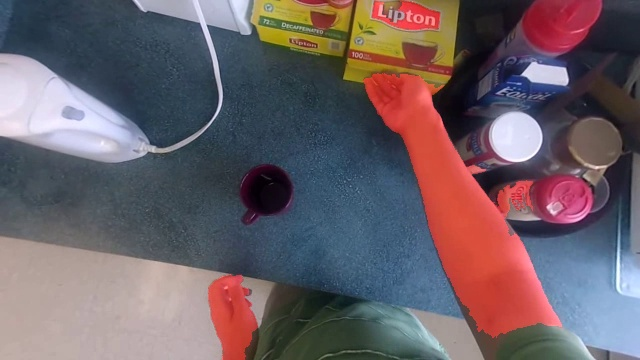
\includegraphics[width=.45\columnwidth]{./Figures/context-free2.jpg}
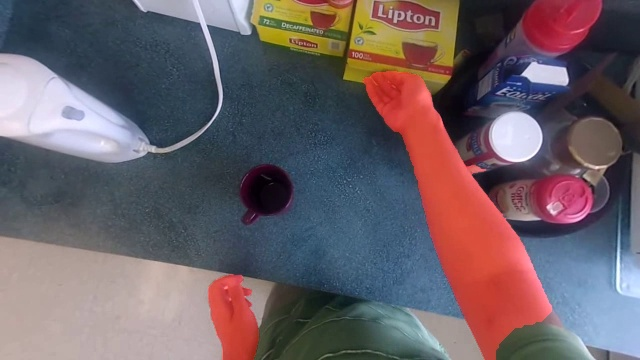
\includegraphics[width=.45\columnwidth]{./Figures/context-dependent2.jpg}
\caption{Comparison before (left image) and after (right image) Temporal smoothing.}
\label{fig:gesture_samples_time}
\end{figure}
Temporal smoothing aims to improve the foreground prediction of a pixel in a frame by a weighted combination of
its previous frames, since past frames should affect the results prediction for the current frame. This technique is inspired by \cite{liu08}.

The smoothing filter for a pixel $\mathbf{x}_{t}^{i}$ of a frame $t$  can thus be defined as follows:

\begin{multline}
P(\mathbf{x}_{t}^{i}=1) = \sum_{k = 0}^{\min(d,k)} w_{k} \bigl( P(\mathbf{x}_{t}^{i}=1|\mathbf{x}_{t-k}^{i}=1) \cdot P(\mathbf{x}_{t-k}^{i}=1|\mathbf{l_{t-k}},\mathbf{g_{t-k}})\, + P(\mathbf{x}_{t}^{i}=1|\mathbf{x}_{t-k}^{i}=0) \, \cdot \\
\cdot P(\mathbf{x}_{t-k}^{i}=0|\mathbf{l_{t-k}},\mathbf{g_{t-k}}) \bigr)
\end{multline}
where $P(\mathbf{x}_{t-k}^{i}=1|\mathbf{l_{t-k}},\mathbf{g_{t-k}})$ is the posterior probability
that a pixel in frame $t-k$ is marked as hand part and $d$ is a number of past frames used. This likelihood can be defined as the probability $P(\mathbf{s}|\mathbf{l_{t-k}},\mathbf{g_{t-k}})$, being
$\mathbf{x}_{t}^{i}$ part of $\mathbf{s}$. In the same way, $P(\mathbf{x}_{t-k}^{i}=0|\mathbf{l_{t-k}},\mathbf{g_{t-k}})$ is defined as the probability
$1-P(\mathbf{s}|\mathbf{l},\mathbf{g_{t-k}})$. 

While $P(\mathbf{x}_{t}^{i}=1|\mathbf{x}_{t-k}^{i}=1)$ and $P(\mathbf{x}_{t}^{i}=1|\mathbf{x}_{t-k}^{i}=0)$ are prior probabilities estimated
from the training set as follows:

\begin{equation}
P(\mathbf{x}_{t}^{i}=1|\mathbf{x}_{t-k}^{i}=1)=\frac{\#(\mathbf{x}_{t}^{i}=1,\mathbf{x}_{t-k}^{i}=1)}{\#(\mathbf{x}_{t-k}^{i}=1)}
\end{equation}


\begin{equation}
P(\mathbf{x}_{t}^{i}=1|\mathbf{x}_{t-k}^{i}=0)=\frac{\#(\mathbf{x}_{t}^{i}=1,\mathbf{x}_{t-k}^{i}=0)}{\#(\mathbf{x}_{t-k}^{i}=0)}
\end{equation}


where $\#(\mathbf{x}_{t-k}^{i}=1)$ and $\#(\mathbf{x}_{t-k}^{i}=0)$ are the number of times in which $\mathbf{x}_{t-k}$ belongs or not to
a hand region, respectively; $\#(\mathbf{x}_{t}^{i}=1,\mathbf{x}_{t-k}^{i}=1)$ is the number
of times that two pixels at the same location at frame $t$ and $t-k$ belong to a hand part; 
similarly, $\#(\mathbf{x}_{t}^{i}=1,\mathbf{x}_{t-k}^{i}=0)$
is the number of times that a pixel in frame $t$ belongs to
a hand part and pixel in the same position in frame $t-k$ does not belong
to a hand region. 

Based on our preliminary experiments we set $d$ equal to three.
Figure \ref{fig:gesture_samples_time} shows an example where temporal smoothing deletes blinking regions (i.e. the tea box brand and jar shadows on the right).


\subsection{Spatial consistency}
\begin{figure}[tb]
\centering
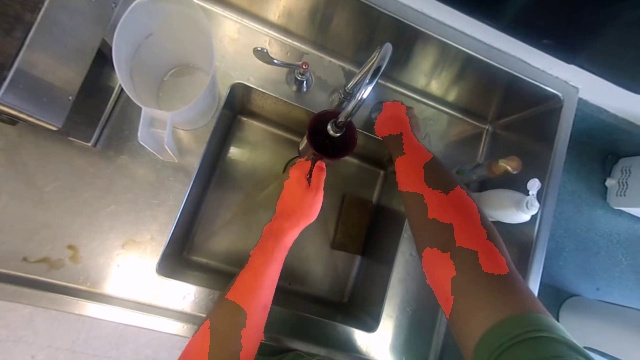
\includegraphics[width=.45\columnwidth]{./Figures/context-free1.jpg}
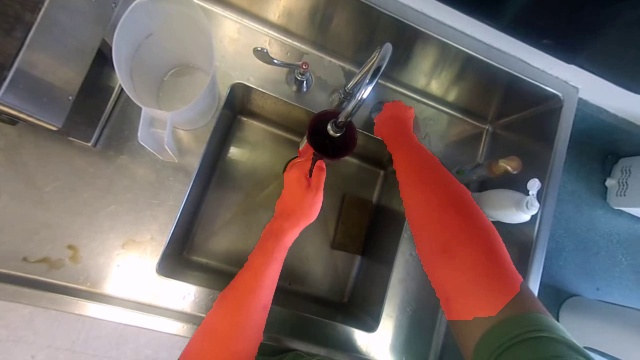
\includegraphics[width=.45\columnwidth]{./Figures/context-dependent1.jpg}
\caption{Comparison before (left image) and after (right image) Spatial Consistency.}
\label{fig:gesture_samples_space}
\end{figure}
Given pixels elaborated by the previous steps, we want to exploit spatial consistency to prune away small and isolated pixel groups that are unlikely to be part of hand regions and also aggregate bigger connected pixel groups. To this aim, we exploit the GrabCut algorithm \cite{rother04}, which essentially works as follows:

\begin{figure}[htbp]
	\centering
		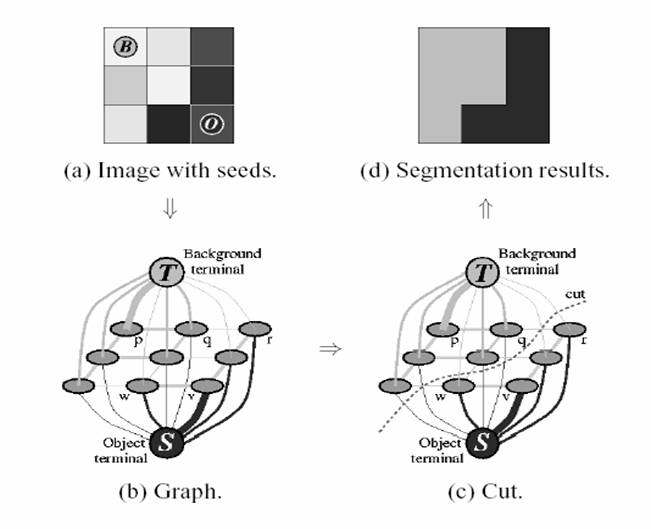
\includegraphics[width=.55\linewidth]{Figures/grabcut.jpg}
	\caption{The GrabCut algorithm.}
	\label{fig:GrabCut}
\end{figure}
 
\begin{enumerate}
\item It takes as input an initial trimap by of background, foreground and unknown pixels.
\item It creates an initial image segmentation, where all unknown
pixels are tentatively placed in the foreground class
and all known background pixels are placed in the background
class.
\item Gaussian Mixture Models (GMMs) are created for initial foreground
and background classes.
\item Each pixel in the foreground class is assigned to the most
likely Gaussian component in the foreground GMM. Similarly,
each pixel in the background is assigned to the most
likely background Gaussian component.
\item The GMMs are thrown away and new GMMs are learned from
the pixel sets created in the previous set.
\item A graph is built and Graph Cut is run to find a new tentative
foreground and background classification of pixels (Fig. \ref{fig:GrabCut}).
\item Steps 4-6 are repeated until the classification converges

\end{enumerate}

For every pixel $\mathbf{x}$, we extract its posterior probability $P(\mathbf{x}_{t}^{i})$ and use it as input for the GrabCut algorithm. Each pixel with $P(\mathbf{x}_{t}^{i}) \geq 0.5$ is marked as foreground, otherwise it's considered as part of background. After the segmentation step, we discard all the small isolated regions that have an area of less than 5\% of the frame and we keep only the three largest connected components.

In Figure \ref{fig:gesture_samples_space} an example with and without applying the Spatial Consistency method is depicted; notice this technique allows to better aggregate superpixels that are near the principal blob region.


\begin{figure*}[tb]
\centering
\subfigure[]{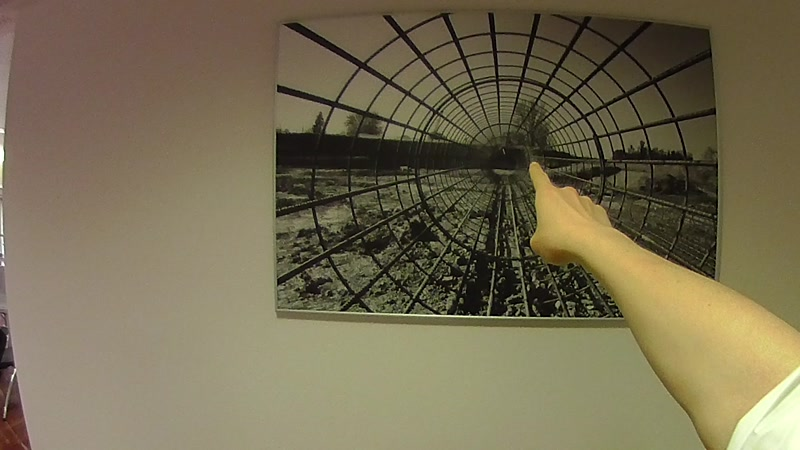
\includegraphics[width=.30\columnwidth]{./Figures/index_sample.jpg}}
\subfigure[]{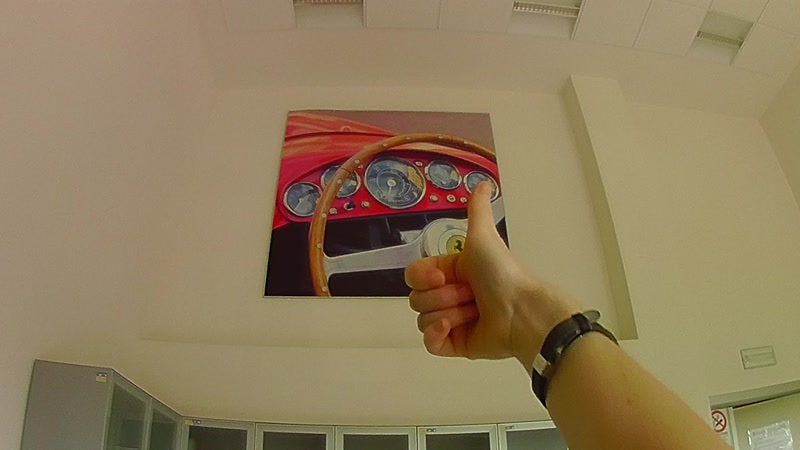
\includegraphics[width=.30\columnwidth]{./Figures/like_sample.jpg}}
\subfigure[]{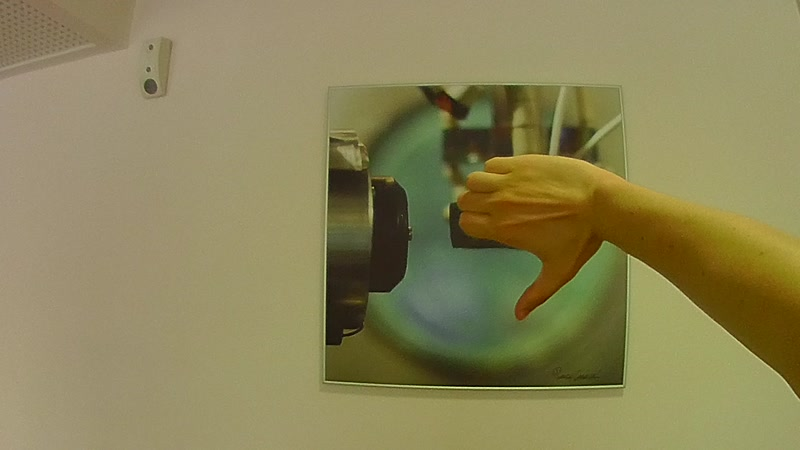
\includegraphics[width=.30\columnwidth]{./Figures/dislike_sample.jpg}}
\subfigure[]{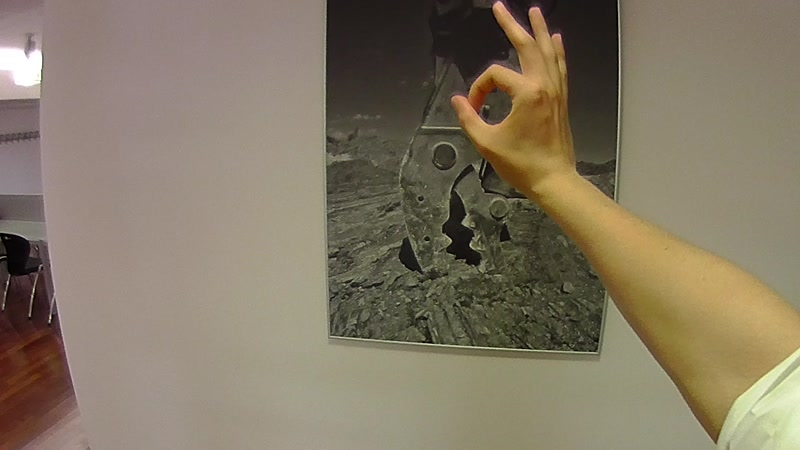
\includegraphics[width=.30\columnwidth]{./Figures/ok_sample.jpg}}
\subfigure[]{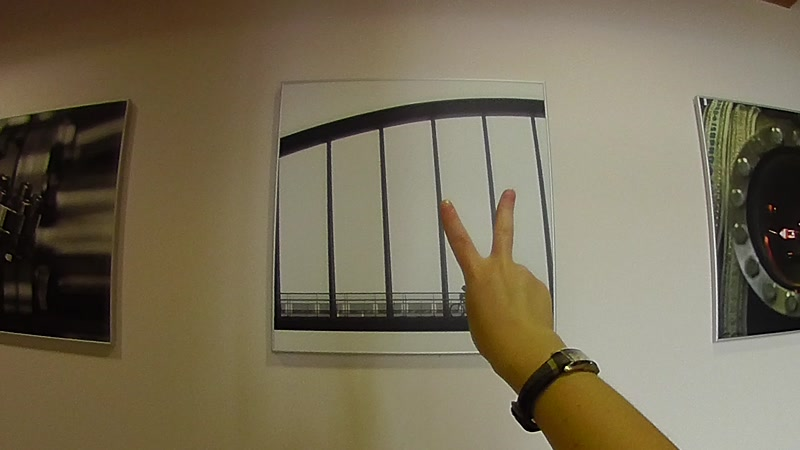
\includegraphics[width=.30\columnwidth]{./Figures/victory_sample.jpg}}
\caption{The EGO-HSGR dataset contains hands performing five gestures: a) point out; b) like; c) dislike; d) ok; e) victory.}
\label{fig:gesture_samples}
\end{figure*}

\section{Experimental results}
Having fully described our method, we now want to evaluate its performance on two datasets: EDSH and EGO-HSGR.
The recent publicly available EDSH dataset \cite{li13} consists in egocentric videos acquired to analyze performance of several hand detection methods. It consists of three videos (EDSH\_1, used as train video, and EDSH\_2 and EDSH\_{kitchen} used as test videos) that contain indoor and outdoor scenes with large variations of illumination, mild camera motion induced by walking and climbing stairs. All videos are recorded at a resolution of 720p and a speed of 30 fps. Also, the dataset includes segmentation masks of hands.    

We also generated a new dataset which contains 12 videos of indoor scenes (EGO-HSGR). Videos have been recorded with a Panasonic HX-A10 Wearable Camcorder (see \ref{panasonic}) at a resolution of $800 \times 450$ with a 25FPS in two different locations: a library and department's exhibition area.   

The aim of this dataset is to reproduce an environment similar to a museum for human and object interaction: paintings and posters are hung on the walls, true masterpieces or either its virtual images; the visitor walks and sometimes stops in front of an object of interest performing some gestures to interact with next generation wearable devices. We identify five different gestures that are used commonly: \textit{point out}, \textit{like}, \textit{dislike}, \textit{ok} and \textit{victory}. These can be associated to different action or used for record social experience. Fig. \ref{fig:gesture_samples} shows some frame examples. 

To evaluate performance of our pixel-level hand detector a subset of six videos are used (three for training and two for testing). Segmentation masks are provided every 25 frames for a total of 700 annotations. 
The F-score (harmonic mean of the precision and recall rate) is used to quantity hand detection performance.
%(we denote these videos as BB\_L1 and BB\_L2), a corridor of a faculty (BB\_F1 and BB\_F2) and a department (BB\_D1 and BB\_D2).

In the following subsections, we are going to evaluate every single aspect of our method: the performance of the features, and of the proposed techniques: temporal consistency, spatial coherence and illumination invariance. We will also compare our approach to existing methods.
    
 \begin{table}
 \centering
 \begin{tabular}{|l|c|c|}
 \hline
 \textbf{Features} 	& \textbf{EDSH\_2} & \textbf{EDSH\_{kitchen}}	\\ \hline\hline
 HSV	& 0.752 & 0.801		\\ \hline
 + LAB	& 0.754	&	0.808 \\ \hline
 + LAB hist.	& 0.755 & 0.823			\\ \hline  
 + HSV hist. & 0.755 & 0.823			\\ \hline  
 + Grad hist. & 0.758	&	0.828	\\ \hline  
 + Gabor & 	\textbf{0.761}	& \textbf{0.829} \\ \hline  
 \end{tabular}
 \caption{Performance by incrementally adding new features.}\label{tab:localfeatures}
 \end{table}

\subsection{Features performance}

First, we examine the effectiveness of our features to discriminate between hand and non-hand superpixels. 
Table \ref{tab:localfeatures} shows performance in terms of F-measure on EDSH dataset with different feature combinations: firstly we describe each superpixel with mean and covariance matrix of its pixel values in HSV colour space, then we do the same using LAB colour space and we add colour histograms. Lastly, we include a histogram of gradients and Gabor feature.
In order to analyze how visual features impact on the performance, in this experiment we do not include the temporal and spatial context information by using a single random forest classifier.     
Note that although colour information plays a fundamental role for hand detection, some ambiguities between hands and other similar coloured object still remain; these can be reduced by adding features based on gradient histograms. In fact, the usage of the full descriptor slightly improves the performance.      

\begin{table}
 \centering
 \begin{tabular}{|l|c|c|}
 \hline
 \textbf{Features} 	& \textbf{EDSH\_2} & \textbf{EDSH\_{kitchen}}	\\ \hline\hline
 II	& 0.789 & 	0.831		\\ \hline
 II + TS	& 0.791	&	0.834 \\ \hline
 II + TS + SC &	\textbf{0.852} &	\textbf{0.901}	\\ \hline  
 \end{tabular}
 \caption{Performance comparison considering Illumination Invariance (II), Time Smoothing (TS) and Spatial Consistency (SC).}\label{tab:context}
\end{table}


\subsection{Temporal Smoothing and Spatial Consistency}
In this experiment we validate the proposed techniques that take into account illumination variations, time dependence and spatial consistency.
Table \ref{tab:context} shows the F-measure scores obtained on EDSH dataset incrementally adding Illumination Invariance (II), Time Smoothing (TS) and Spatial Consistency (SC). 
Note that there is a significant improvement in performance when all these three techniques are applied together.   
In particular, illumination invariance substantially increases the performance with respect to results obtained using only visual features and a single random forest classifier, while the improvement introduced by temporal smoothing is less pronounced. The main contribution is given by Spatial Consistency, that prunes away small and isolated pixel groups and merge spatially nearby regions, increasing the F-measure score of about six percentage points.
The proposed technique is also tested in our EGO-HSGR dataset obtaining an F-measure score of $0.908$ and $0.865$ for the EGO-HSGR\_{4} and EGO-HSGR\_{5} videos.        


\begin{table}
 \centering
 \begin{tabular}{|l|c|c|}
 \hline
  	& \textbf{EDSH\_2}	& \textbf{EDSH\_{kitchen}} \\ \hline\hline
Video stabilization  \cite{hayman03} 	& 0.211 & 0.213		\\ \hline
Single pixel colour \cite{jones99}	& 0.708 &	0.787	\\ \hline  
Collection of random forest \cite{li13} & 0.835 & 0.840		\\ \hline  
\textbf{Our method} & \textbf{0.852} &	\textbf{0.901}	\\ \hline 
\end{tabular}
\caption{Hand segmentation comparison with the state-of-the-art.}\label{tab:comparision_hand}
\end{table}



\subsection{Comparison to related methods}

In Table \ref{tab:comparision_hand} we compare our results to several approaches on EDSH dataset: a single-pixel colour approach inspired by \cite{jones99}, a video stabilization approach based on background modeling using affine alignment of image frames inspired by
\cite{hayman03} and the approach based on random forest, by Li \etal \cite{li13}. 
The single-pixel approach is a random regressor trained only using single-pixel LAB colour values. 
The background modeling approach aligns sequences of 15 frames estimating their mutual affine transformations; pixels with high variance are considered to be foreground hand regions. 
As can be seen, although the single-pixel approach is conceptually simple, is still quite effective. In addition, we observe that the low performance of the video stabilization approach is due to large ego-motion because the camera is worn by the user.     
The method recently proposed by \cite{li13} is more similar to our approach, but the use of superpixels, the selection of a new set of local features and the introduction of temporal and spatial consistency allow us to outperforms that results.

\medskip
We have addressed one of the main issues involved in hand gesture recognition: hand segmentation. The proposed algorithm will be exploited in the next chapter, where our gesture recognition approach will be introduced and fully described.
